\documentclass[a4paper]{article}
\usepackage[margin=1in]{geometry}

\usepackage[english]{babel}
\usepackage[utf8]{inputenc}
\usepackage{amsmath}
\usepackage{graphicx}
\usepackage[colorinlistoftodos]{todonotes}
\usepackage{float}
\usepackage{tikz}

\title{Bubble Beam - Assignment 5}

\author{
    Bavdaz, Luka\\
    \texttt{4228561}
    \and
    Clark, Liam\\
    \texttt{4303423}
    \and
    Gmelig Meyling, Jan-Willem\\
    \texttt{4305167}
    \and
    Hoek, Leon\\
    \texttt{4021606}
    \and
    Smulders, Sam\\
    \texttt{4225007}
}

\date{\today}

\begin{document}

\maketitle

% ==========================
% Background immage
% ==========================
\tikz[remember picture,overlay] \node[opacity=0.08,inner sep=0pt] at (current page.center){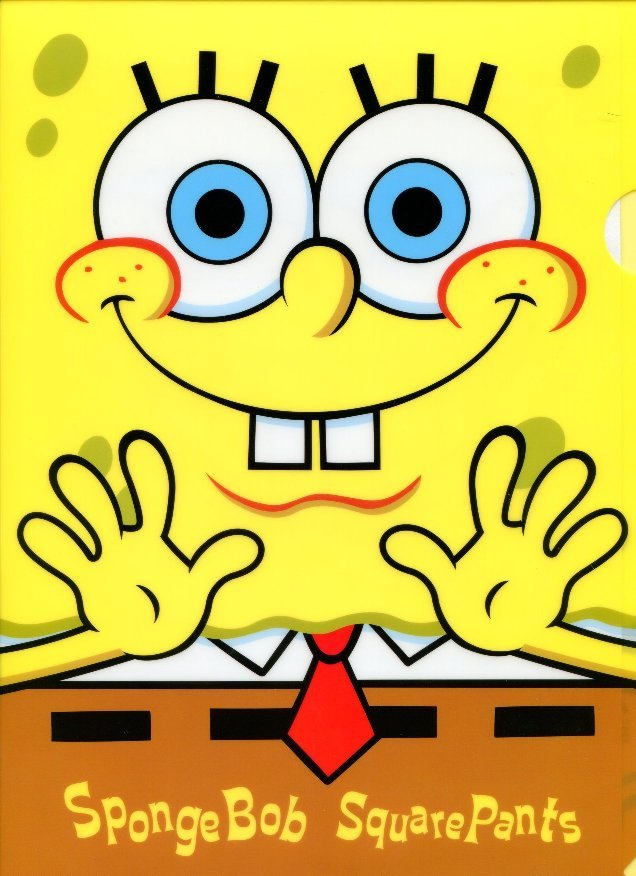
\includegraphics[width=\paperwidth,height=\paperheight]{3368_pd952179_1.jpg}};
\clearpage

% ==========================
% Background immage
% ==========================

\section{20-Time, revolutions}

% ==========================
%  MULTIPLE GAME MODES
% ==========================
\subsection{Multiple game modes}
In the previous sprint we introduced serveral game modes (from requirements \texttt{M-191} to \texttt{M-194}). A Game Mode basically defines what kind of bubbles a player can receive in his cannon. We have implemented several \textit{Power-up Bubbles} (bubbles with a special effect). These Bubbles are constructed through a \texttt{BubbleFactory}, and the Game Mode was basically implemented by providing the \texttt{GameController} with another \texttt{BubbleFactory}.

\par{}Ofcourse it is a bit ambigious to let the \texttt{BubbleFactory} be the object that decides the \texttt{GameMode}. It also was a bit limited: we could provide new bubbles, but a more advanced game mode - Timed Game Mode (\texttt{M-193}) - actually failed because we had no possibility to hook on to the required methods - translating the bubbles - and events - time.

\par{}Speaking of events, over time, the game controller logic became a bit cluttered, after adding hooks and observers/listeners in various ways. Thus, in this sprint, we refactored the event handling system as a starting point for the more advanced game modes and multiplayer improvements.

% ==============================
% 	EVENT HANDLING
% ==============================
\subsubsection{Event handling}
\label{sec:evthdl}

We already use event handling a lot: the \texttt{CannonController} triggers a \texttt{CannonShootEvent} (which is itself most likely triggered by an \texttt{MouseEvent}). The \texttt{GameController} listens for this \texttt{CannonShootEvent} and then starts doing its responsibility: allow the \texttt{MovingBubble} to move and check if it collides with other bubbles on its way, and if so, handle this collision in terms of snapping to the \texttt{BubbleMesh}, or popping with other bubbles.

\par All these actions are in fact events as well, and provide perfect hooks for game mode implementations and  synchronization in the multiplayer. However, in the current version, this eventing system was just not complete enough to make this true. Luckily, the changes do not require a lot of new classes to be introduced, but rather requires to move around a few methods between classes and update their callers.

\subsubsection*{BubbleMesh}
The \texttt{BubbleMesh} is a data structure for the \texttt{Bubbles}, and this structure needs to be maintained as bubbles gets snapped in to the mesh, popped, or inserted at the top. These events can be useful, as points need to be rewarded when bubbles pop. Also, when rows get inserted to the mesh, we want to send this to a potential multiplayer client.

\begin{figure}[H]
    \begin{center}
    \begin{tabular}{ | p{8cm} | p{4cm} | }
      \multicolumn{2}{c}{\texttt{BubbleMesh}} \\ \hline
      \textbf{Responsibilities} & \textbf{Collaborations} \\ \hline
      Datastructure containing the bubbles & \texttt{Bubble} objects \\
      Logic to insert a new row of bubbles & \texttt{BubbleMeshListener} \\
      Logic to snap a bubble into the mesh & \\
      Logic to see if a snap caused any pops & \\
      Notify \texttt{BubbleMeshListeners} of above events & \\
      \hline
    \end{tabular}
    \end{center}
    \caption{CRC-Card for the \texttt{BubbleMesh}}
\end{figure}

\begin{figure}[H]
    \centering
	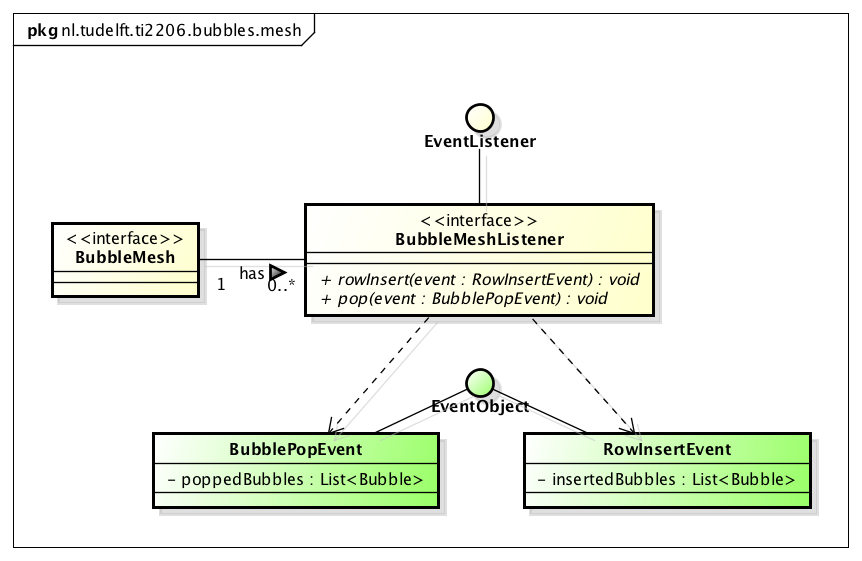
\includegraphics[scale=0.5]{BubbleMeshListener.png}
    \caption{UML Diagram for the \texttt{BubbleMeshListener}}
\end{figure}


\subsubsection*{CannonController}
The \texttt{CannonController} is responsible for the cannon specific logic. It triggers an event when the cannon shoots, which for example is necessary for the \texttt{GameController} to start translating the shot bubble.

\begin{figure}[H]
    \begin{center}
    \begin{tabular}{ | p{8cm} | p{4cm} | }
      \multicolumn{2}{c}{\texttt{CannonController}} \\ \hline
      \textbf{Responsibilities} & \textbf{Collaborations} \\ \hline
      Updating the \texttt{CannonModel} when the cannon rotates & \texttt{Cannon} instance \\
      Preventing new shoot while shooting & \texttt{CannonModel} \\
      Propagating \texttt{ShootEvent} to the \texttt{CannonListeners} & \texttt{CannonListener} \\
      \hline
    \end{tabular}
    \end{center}
    \caption{CRC-Card for the \texttt{CannonController}}
\end{figure}

\begin{figure}[H]
    \centering
    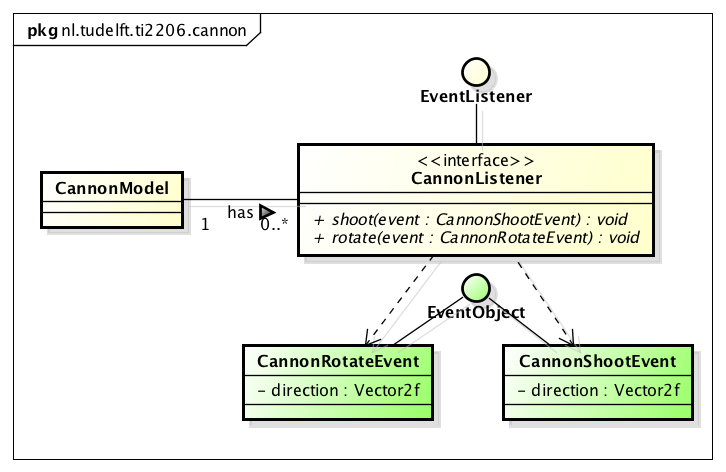
\includegraphics[scale=0.5]{CannonListener.png}
    \caption{UML Class diagram for the \texttt{CannonListener}}
\end{figure}

\clearpage
% = = = GameController
\subsubsection*{GameController}
The \texttt{GameController} is responsible for the generic game logic. See also the following CRC-card:

\begin{figure}[H]
    \begin{center}
    \begin{tabular}{ | p{8cm} | p{4cm} | }
      \multicolumn{2}{c}{\texttt{GameController}} \\ \hline
      \textbf{Responsibilities} & \textbf{Collaborations} \\ \hline
      Check collisions shot bubble & \texttt{BubbleMesh} \\
      Update cannon ammunition & \texttt{CannonController} \\
      Keep track of remaining colours & \texttt{GameListener} \\
      Game Over handling & \\
      Notify \texttt{GameListeners} of above events & \\
      Propagate \texttt{ShootEvents} and \texttt{BubbleMeshEvents} & \\
      \hline
    \end{tabular}
    \end{center}
    \caption{CRC-Card for the \texttt{GameController}}
\end{figure}

\begin{figure}[H]
    \centering
    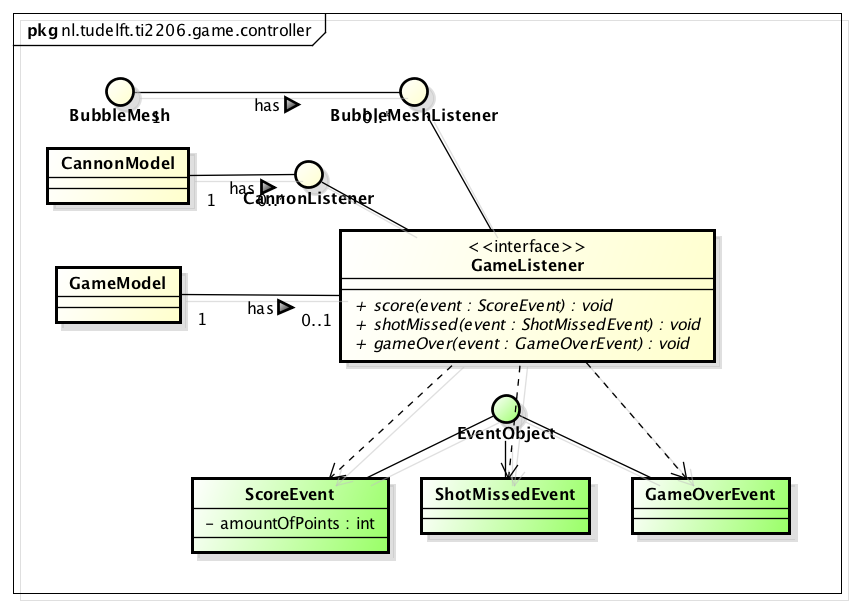
\includegraphics[scale=0.5]{GameListener.png}
    \caption{UML Diagram for the \texttt{GameListener}}
\end{figure}

% ========================
% GAME MODE 
% ========================
\subsubsection{Game Mode}
\label{sec:gmmde}
From the requirements \texttt{M-191} to \texttt{M-194} we expect a \texttt{Game Mode} to have the following abilities: (1) it should be able to provide a certain \texttt{BubbleFactory} to the \texttt{GameController}, so that it can create the correct ammunation for the game mode; (2) it should be able to listen for \texttt{GameEvents}, for example to award points or insert new bubbles after a few misses; and (3) it should be able to listen on \texttt{GameTicks} to perform changes over time, such as pushing bubbles slowly to the bottom in the timed mode. Furthermore, we need to have access to the \texttt{GameController} to invoke these actions, and we also need to add some calls to the \texttt{GameModel} in the \texttt{GameController}.

\begin{figure}[H]
    \begin{center}
    \begin{tabular}{ | p{8cm} | p{4cm} | }
      \multicolumn{2}{c}{\texttt{GameMode}} \\ \hline
      \textbf{Responsibilities} & \textbf{Collaborations} \\ \hline
      Provide a \texttt{BubbleFactory} & \texttt{BubbleFactory} \\
      Listen for \texttt{GameEvents} & \texttt{GameController} \\
      Interact with \texttt{BubbleMesh} & \texttt{BubbleMesh} \\
      Interact with \texttt{GameControler} & \texttt{GameTick} \\
      Ability to hook onto \texttt{GameTicks} & \\
      \hline
    \end{tabular}
    \end{center}
    \caption{CRC-Card for the \texttt{GameMode}}
\end{figure}

Since we want a \texttt{GameMode} to hook onto \texttt{GameEvents}, we decided it should be a \texttt{GameListener}. Because we also want to hook on \texttt{GameTicks}, we decided a \texttt{GameMode} should also be \texttt{Tickable}. For the \texttt{BubbleFactory} and name of the \texttt{GameMode}, we defined getters in the \texttt{GameMode} interface.

\begin{figure}[H]
	\centering
	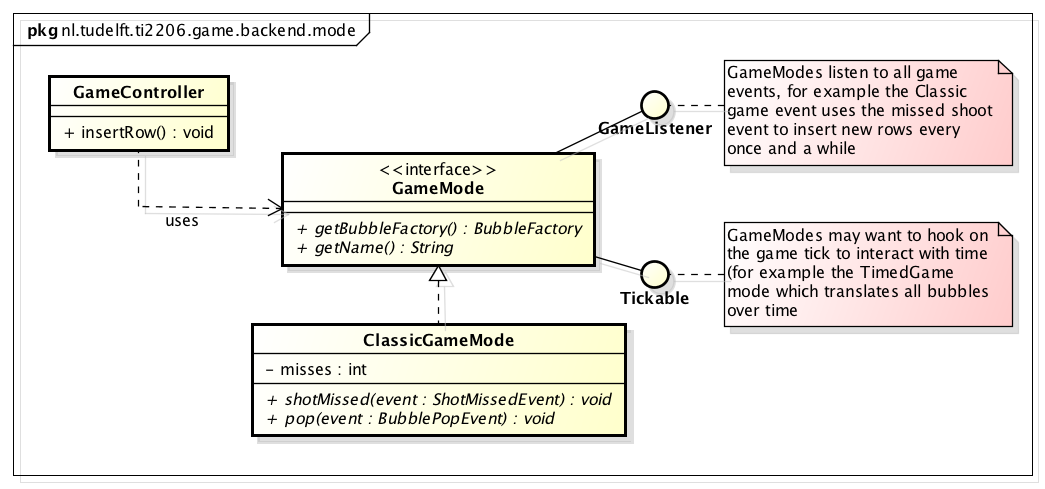
\includegraphics[scale=0.5]{GameMode.png}
    \caption{UML class diagram for the \texttt{GameMode}}
\end{figure}

\subsubsection*{Interactions}
The \texttt{ClassicGameMode} provides bubbles through the \texttt{DefaultBubbleFactory} (which creates only \texttt{ColouredBubbles} and no Power-up bubbles), this is provided through the \texttt{getBubbleFactory} method. When bubbles pop, the player is awarded some points. This is achieved by overriding the \texttt{pop} method from the \texttt{GameListener}. When a shot bubble snaps into the \texttt{BubbleMesh} without popping, it is concidered a miss. After a few misses, a new row is inserted. The same as with the pop, this is done by implementing the \texttt{shotMissed} method. See also the sequence diagram \ref{fig:seqgamemode} for these interactions between the \texttt{GameMode} and the \texttt{GameController}.

\begin{figure}[H]
	\centering
	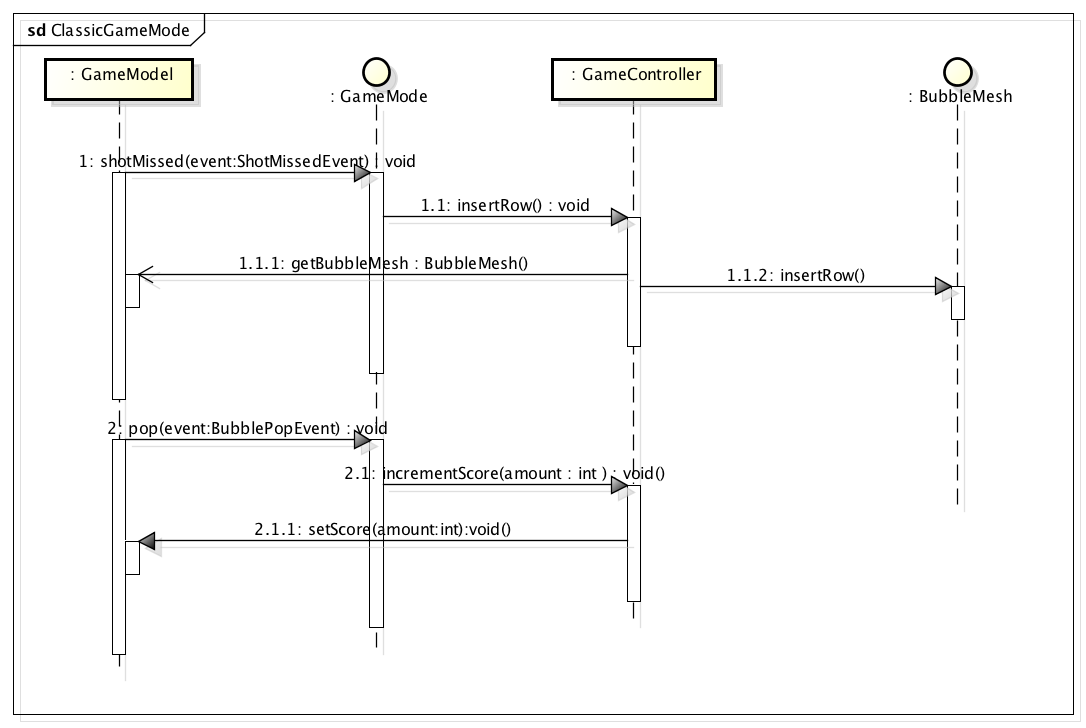
\includegraphics[scale=0.5]{ClassicGameMode.png}
    \caption{UML sequence diagram for the \texttt{GameMode}}
    \label{fig:seqgamemode}
\end{figure}

% ==============================
% 	BUBBLE MESH IMPROVEMENTS
% ==============================
\subsubsection{BubbleMesh improvements}
In the previous iteration a \texttt{Bubble} knew its position and was able to paint itself on a \texttt{Graphics} object. In the \texttt{paintComponent} function of the \texttt{GamePanel} we iterate over all bubbles in the \texttt{BubbleMesh}, and invoke the \texttt{render} method.
For the \texttt{TimedGameMode}, this was not enough. In the \texttt{TimedGameMode} we want all bubbles to slowly fall down at a certain speed. When they reach the bottom, the game is over, or when the \texttt{BubbleMesh} is empty, you have defeated the game mode. We needed to be able to translate the entire \texttt{BubbleMesh}.

\begin{figure}[H]
	\centering
	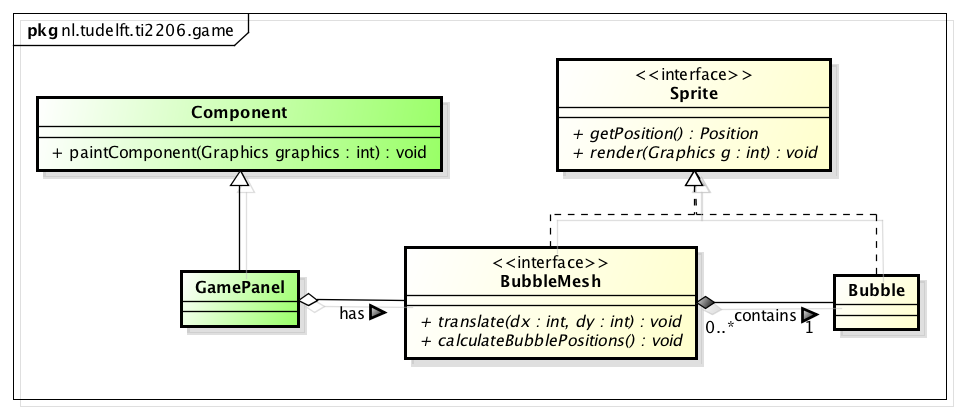
\includegraphics[scale=0.5]{BubbleMeshSprite.png}
    \caption{UML class diagram for the \texttt{BubbleMesh} }
    \label{fig:bmeshsprite}
\end{figure}

We figured out that it would be more clear to let the \texttt{BubbleMesh} be a \texttt{Sprite} as well, and give it the ability to draw itself and its bubbles. Then the \texttt{GamePanel} calls the render method of the \texttt{BubbleMesh} instead of the induvidual bubbles. Also we gave the \texttt{BubbleMesh} a position which can be translated - also moving the bubbles in the \texttt{BubbleMesh}.

\par{} With these adjustments to the \texttt{BubbleMesh} and the event listener changes described in section \ref{sec:evthdl} and \ref{sec:gmmde}, we now have all the ingredients to make the \texttt{TimedGameMode} work: in the \texttt{GameMode} we can now hook onto the \texttt{GameTick} and then slightly translate the \texttt{BubbleMesh}.

% ==============================
% 	GAME MODES FOR MULTIPLAYER
% ==============================
\subsubsection{Game modes for multiplayer}
In the previous version we only transmitted the \texttt{CannonEvents} and some \texttt{BubbleMesh} syncs, and let the client then guess what other events might have been triggered. Also, we just hardcoded to always pick the \texttt{PowerUpBubbleFactory} (so what now would be the \texttt{PowerUpGameMode}). This did not give us the ability to play other \texttt{GameModes}, or use any of the Game Mode logic introduced in section \ref{sec:gmmde}.

\par{}Therefore we decided to rework the multiplayer. First, when we create a room (player 1 clicks "start multiplayer"), we want to be able to select one of the \texttt{GameModes}. Then we want to create two \texttt{GameModels} with this \texttt{GameMode} and an initial \texttt{BubbleMesh} and ammunition \texttt{Bubbles}. When a client connects (player 2 clicks "find multiplayer"), we need to transmit and process this initial data.

\begin{figure}[H]
	\centering
	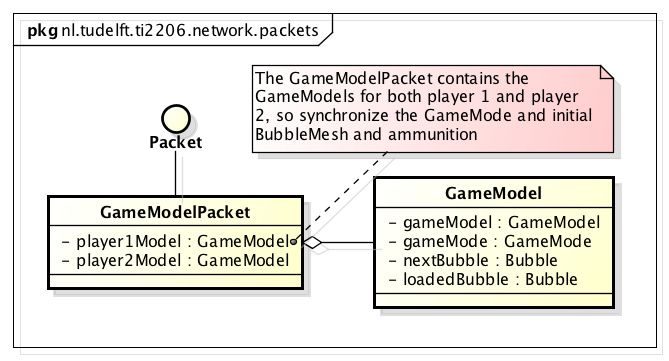
\includegraphics[scale=0.5]{GameModelPacket.png}
    \caption{UML class diagram for the \texttt{GameModelPacket} }
    \label{fig:gmpacket}
\end{figure}

After transmitting the \texttt{GameModelPacket} both players can start playing. Now we need to transmit all actions between the two clients. In the previous version we used some dedicated packets for this, but the implementation was incomplete. Now we have an advanced event handling system (section \ref{sec:evthdl}), and all we have to do is listen for a \texttt{GameEvent} being triggered in the active game panels, wrap it in an \texttt{EventPacket}, transmit it to the client (figure \ref{fig:connectorgamelistener}).

\begin{figure}[H]
	\centering
	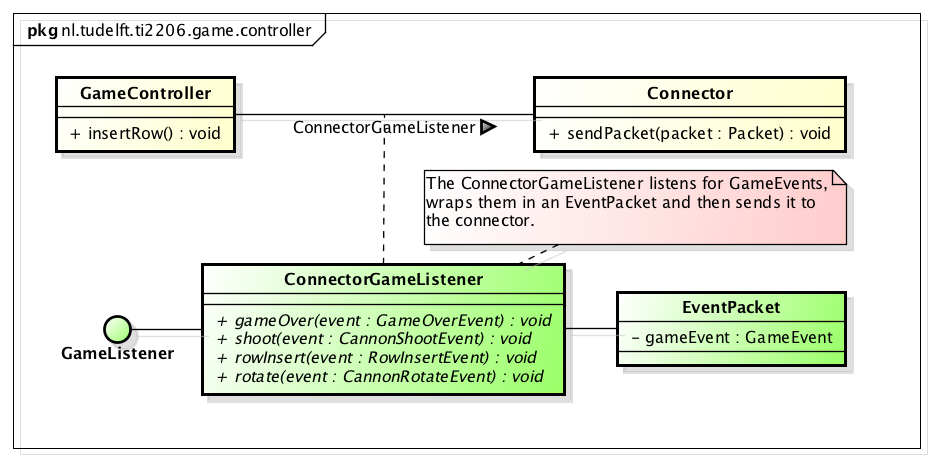
\includegraphics[scale=0.5]{ConnectorGameListenerExtended.png}
    \caption{UML class diagram for the \texttt{ConnectorGameListener} }
    \label{fig:connectorgamelistener}
\end{figure}

When the client receives an \texttt{EventPacket}, it needs to update the \texttt{GameController}. Therefore we have made a \texttt{PacketListener} that listens for \texttt{EventPackets}, and then invokes the event on the \texttt{GameController} (figure \ref{fig:slavegamepacketlistener}).

\begin{figure}[H]
	\centering
	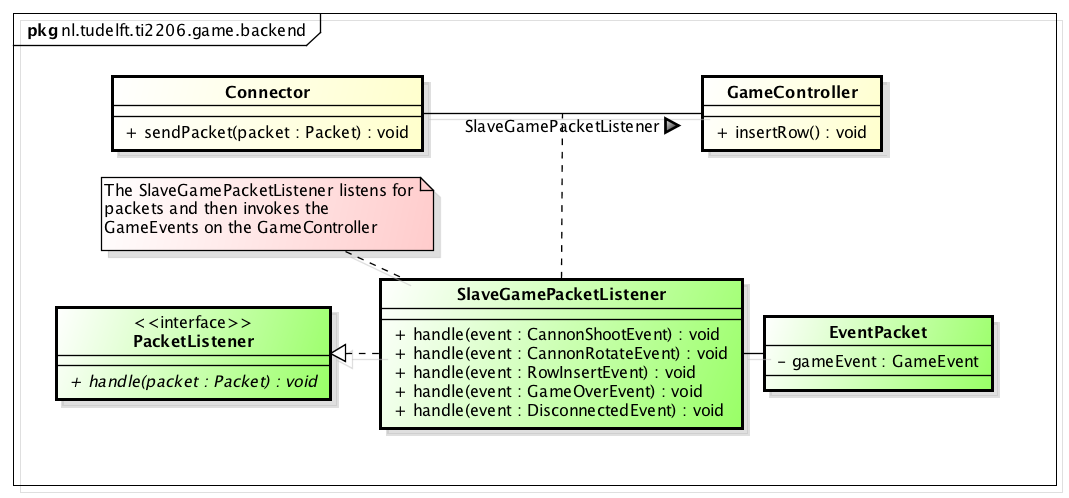
\includegraphics[scale=0.5]{SlaveGamePacketListener.png}
    \caption{UML class diagram for the \texttt{SlaveGamePacketListener} }
    \label{fig:slavegamepacketlistener}
\end{figure}

Now we have access to all required events in the multiplayer, which also allows the \texttt{GameModes} to work completely in multiplayer.


% ==============================
% 	POP ANIMATIONS
% ==============================
\subsection{Pop animations}
In the prvious sprint we already implemented two pop animmations for our requirement \texttt{C-193}, "When a bubble is popped, a pop animation should be played". But we could only play a the same pop animation for all bubbles. In this sprint we want to add multiple pop animations and give different bubbles different animations.

We already developed a \texttt{FallDownAnimation} and a \texttt{ShrinkAnimation}. We decided to give all normal bubbles the \texttt{ShrinkAnimation} and the \texttt{StoneBubble} the \texttt{FallDownAnimation}. For our \texttt{JokerBubble} we added the \texttt{ConfettiAnimation} class and for the \texttt{BombBubble} the \texttt{ExplosionAnimation} class.

To use different bubble animations for different bubbles we had to add a way to get the animation from the bubble. Therefore we added a method in the \texttt{Bubble} interface: \texttt{getAnimation() : FiniteAnimation}. In this method a \texttt{Bubble} returns the corresponding animation for when the (decorated) bubble pops. We also changed the way the animations are added to the game panel, we nog use the getAnimation method to get the annimation to be added. See Figure \ref{fig:addPopAnimations}.

\begin{figure}[H]
	\centering
	\begin{tabular}{ | p{8cm} | p{4cm} | }
      \multicolumn{2}{c}{\texttt{Bubble}} \\ \hline
      \textbf{New Responsibilities} & \textbf{New Collaborations} \\ \hline
      Logic to create a new  \texttt{FiniteAnimation} on request & \texttt{FiniteAnimation} \\
      \hline
    \end{tabular}
    \caption{CRC-card for the \texttt{Bubble}}
\end{figure}

%
%	NOTE
%		As nothing changed here since the previous version,
%		I suggest to leave this out of the RDD document (JW)
%
% \begin{figure}[H]
%	\centering
%\begin{tabular}{ | p{8cm} | p{4cm} | }
%      \multicolumn{2}{c}{\texttt{GamePanel}} \\ \hline
%      \textbf{New Responsibilities} & \textbf{New Collaborations} \\ \hline
%      Requesting the \texttt{FiniteAnimation} for each popped bubble & \texttt{FiniteAnimation}  \\
%      \hline
%    \end{tabular}
%    \caption{CRC-card for the \texttt{GamePanel}}
%\end{figure}

\begin{figure}[H]
	\centering
	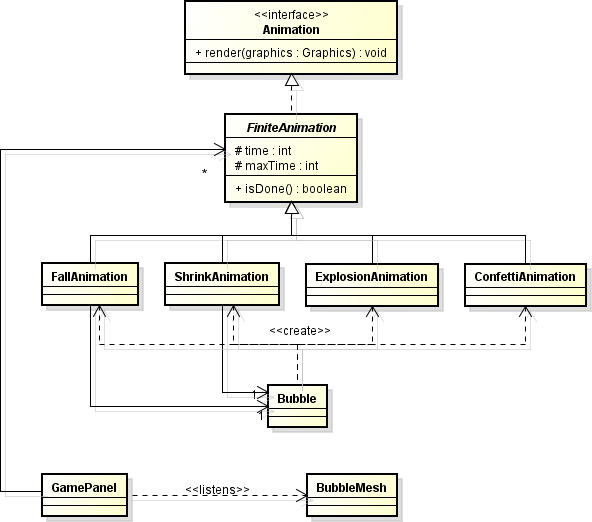
\includegraphics[scale=0.4]{newAnimationClassDiagram.png}
    \caption{UML class diagram for the annimations }
    \label{fig:newAnimationClassDiagram}
\end{figure}
\begin{figure}[H]
	\centering
	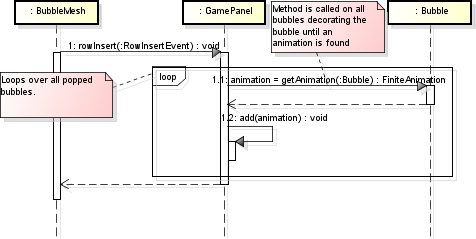
\includegraphics[scale=0.8]{addPopAnimations.png}
    \caption{UML class diagram for the annimations }
    \label{fig:addPopAnimations}
\end{figure}

% ==============================
% 	MULTIPLE LEVELS
% ==============================
\subsection{Multiple levels in game modes}

According to requirement \texttt{M-128} we want new levels (new maps of bubbles) to appear when a player finishes in the singleplayer mode (requirement \texttt{M-127}). In the previous version we could already load a specific \texttt{BubbleMesh} from a text file, but we only used this for the default map. In this version, we updated the game to support a variety maps.

\par{} First, we enrichted the \texttt{GameMode} with two new methods: \texttt{hasNextMap} and \texttt{getNextMap}. This basically makes the \texttt{GameMode} an \texttt{Iterator}. Each \texttt{GameMode} should at least provide one map through these methods, but has the ability to provide more maps.

\par{} Then we needed to call these methods to actually use the maps. This was a bit more difficult: in order to create a game, we first create a \texttt{GameModel} with a \texttt{BubbleMesh}. Therefore it already needs to have the \texttt{BubbleMesh} while we yet do not have access to the \texttt{GameController} nor the \texttt{GameMode} instance - which lives in the \texttt{GameController}.

\par{} Therefore we changed the design a bit. The \texttt{GameModel} contains the \texttt{BubbleMesh}, but not necessarily has to be instantiated with it. It is then provided through the \texttt{GameController}, which also has the ability to reload it when the game is won. See also the sequence diagram in figure \ref{fig:GameModeMap}.

\begin{figure}[H]
	\centering
	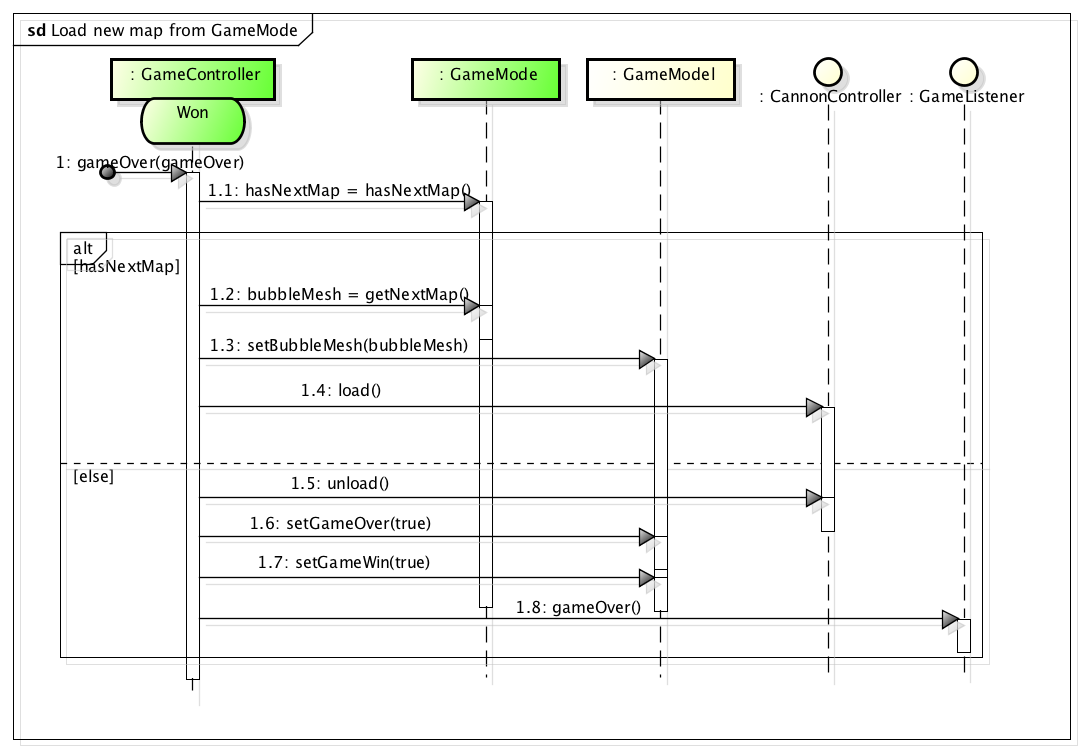
\includegraphics[scale=0.4]{GameModeMap.png}
    \caption{Sequence diagram for retrieving the next map for the game}
    \label{fig:GameModeMap}
\end{figure}

% ==============================
% 	GUI IMPROVEMENTS
% ==============================
% \subsection{GUI Improvements}

% NOTE
%	Since these changes probably aren't to drastic to the
%	structure of the program, we may concider to not
%	describe it in the RDD document (JW)

% ==========================
% WRAP UP REFLECTION
% ==========================
\clearpage
\section{Wrap up - Reflection}
%Blablabla, - > projet done, great results

In the next paragraphs we will take a look on our progress and what we have learned during this project and course. We will discuss how using Scrum helped us to manage this project, what we have learned about ourselves as a team, how the use of design patterns influenced the project and helped us developing and finally we will look back at the beginning of the project.

% ==========================
% Desgin Patterns
% ==========================
\subsection{Design Patterns}
Design patterns have been really valuable to our project. Some complex problems could easily be solved by implementing a design pattern. These design patterns improved our overal code quality, gave our project some structure and also made it easier to extend our game.

Another big advantage was that the code was easier to understand for other project members because of the predefined way the design patterns should work. In combination with the UML and Javadoc it was easier to understand the work of others, without needing to ask them for their explanation.

The code quality was for example improved by implementing the state pattern for the cannon. This design pattern prevented many if-statements and resulted in better organized state handling.

The power-ups, for example, would have been implemented with one class for each combination of power-ups, which are resposible for all the behaviour. With the decorator pattern we where able to split the responsibilities and combine multiple power-ups, like the SoundBubble and DrunkBubble. This made it easier to add new power ups and prevented a complicated inherentance or copying a lot of code.

By applying the factory method for generating bubbles, multiple game modes could be easily added to extend the game without needing a large generation method with many if-statements.

We will definitely use design patterns in our future projects. During this project the design patterns proved themselves most useful. Furthermore, in future projects design patterns can be used from the beginning to provide an effective structure for the rest of the code.

\subsection{What we have learned about ourselves as a team}
We have learned the importance of UML and documentation in general. It is very useful and necessary for communicating with team members about changes team members have made to the code. We learned that every team member has different strenghts, which could all be applied to different parts of the project. 

We have also learned that it is difficult to work on an expanding project without getting overwhelmed by its growing complexity. Even though the design patterns brought some much needed clarity in our code we realized that we were spending a significant amount of time just reading the code to keep our understanding of the project up to date. That is a big difference compared to the smaller projects we did up until now. Now that we have completed this project we can be confident in ourselves that we have the tools and knowledge to tackle even bigger projects.

\subsection{Practical Scrum}
We highly valued the use of Scrum in our project. The methodology enforces a very task-based approach, which in our project lead to a very clear distribution of tasks. This is a good thing in any project because it gets rid of the "I don't know what I should do"-overhead. We also experienced Practical Scrum as a way to prevent a loss of focus inside our team when team members had different visions about what the next step in our project should be. We were forced to decide as one unit what the next course of action should be.

The weekly reflection on the previous sprint was an important tool in creating the next sprint. They were a great reference for how much we could do in a week's time. They also showed what areas still needed attention. Considering Scrum has become the industry-standard over the past few years, learning how to do it properly is a great step forward for all of us. We will use this methodology a lot in the coming years and are confident in our ability to use its strenghts to the fullest.

\subsection {Evolution of the code}
The code for BubbleBeam has come a long way since the first version. An enormous amount of features has been added, yet not in a way that endangered code quality or performance. During the development stages we have seen our simplistic game transform into a content-rich, strongly themed and noteworthy game. To be proud of the final product is a pleasant feeling for any software developer and we would like to share some of our story.

\subsubsection{The intial sprint}
The first part of development is always challenging. We had to decide what to build. We had tons of ideas, yet they had to be organized neatly in our requirements document. Many discussions were held whether something should be a must have or a should have, how to correctly phrase a requirement so that it is not too ambiguous and not in conflict with other requirements to ensure both developers and stakeholders understand and can agree on them. This was a new concept to us so we took our time for this and made sure the requirements were solid before we started programming. 

One of the cornerstones Classes of the project was made during this phase, namely the \texttt{BubbleMesh}. The \texttt{BubbleMesh} class takes care of storing the bubbles and executing the logic of popping bubbles. At this stage this class was not perfect yet but it would soon become a solid foundation for the rest of the project.

All basic functionality was added during this phase but alot of classes had multiple responsibilities. For instance, the class \texttt{Cannon} had to do gamelogic, graphics and user input.

\subsubsection{Assignment 1-2 -refactor}
We had to look back at our initial product and spot its flaws. We found classes with multiple responsibilities, bugs and missing requirements. We modelled the weak and cluttered parts of our code. Having a new arsenal of freshly learned design patterns we decided to tackle these problems. We chose to fix the issues with fitting design patterns, consisting of but not limited to: Observer, MVC and Strategy.

During this sprint and the next a lot of bug-hunting was done and many bugs were found. We made a logger to provide us with the vital information needed about the program, to find and solve more and more bugs.

We ran into major trouble with the multiplayer mode. There was not enough time to do it the way we wanted to do it. So we chose to make a more basic play-together mode first. Then in next few sprints we refactored the multiplayer mode the way it was defined in the requirements document.

\subsubsection{Assignment 3 -Test it}
	With a solid foundation in place, the feature creep could start. We gave the game a solid theme and used more patterns to create more features while trying to maintain a clear control flow of the code. good sprint management was essantial here. We were lacking behind in the  testing department so time was allocated in the plan to make up for this.
 we quickly achieved around 60\% code coverage. and planned in more time in further sprint to up this to.
 
 % The oracle has spoken?
 \subsubsection{Assigment 4 -Incode the oracle hath speaketh
 }
 It was time to put our code quality to the test. Incode had to be run and with pleasing results. Incode discovered only two violations. The design patterns had kept coupling of classes and multiple responsibilities to a minimum.
 Besides fixing the violations we also upped the test coverage to around 85\% for non-gui classes. But mostly this phase was about perfecting and reapplying what we learned earlier, to perfect the art.
 
 \subsubsection{Assignment 5 -The final stretch}
 The final phase of development were upon us, here we mostly polished the product we strenghted the theme with music, more animations and an overal better UI. We also implemented the pre-designed levels. We ensured it is a game we are proud of and that it represents what we have learned. We hope that everyone who plays this game will derive as much joy from it as we did!

\end{document}